<<<<<<< Updated upstream
\section{Conventional Boost Converter}\label{ch:CBC}
\todo[color=c04a,inline]{Conventional Boost Converter}
=======

\subsection{Principle of operation}\label{sec:SON}

The conventional boost converter uses one inductor,
one switch and one capacitor. When the switch is closed, the inductor current rises and energy is stored in the inductor L. When the switch is open, the inductor discharges through diode D and the inductor current falls. It steps up the voltage when
the switch is in OFF state. The two modes of operation will be discussed in this chapter. The circuit can be observed on figure..


\begin{figure}[H]
   \centering
   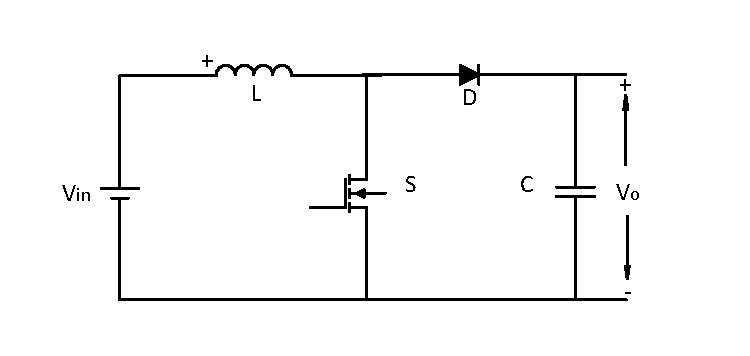
\includegraphics[width=\textwidth]{figures/aConventionalBoost/ConventionalBoostConverter.pdf}
    \caption{Conventional Boost Converter}
	\label{fig:ConventionalBoost}
\end{figure}

\subsection{Operation Modes}\label{sec:SON}

Switch ON:

When the switch is ON,
the inductor is being charged and the capacitor discharges over the load resistor.

\begin{figure}[H]
   \centering
   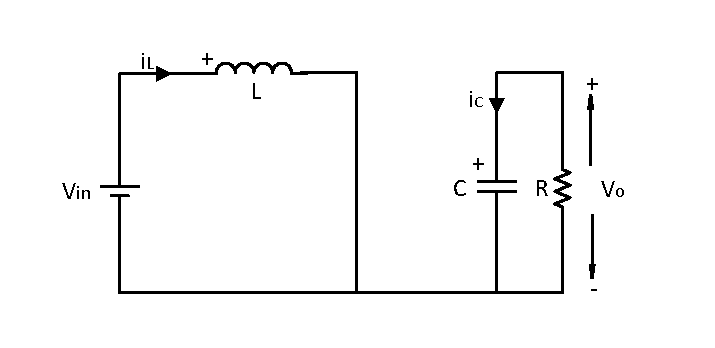
\includegraphics[width=\textwidth]{figures/aConventionalBoost/ConventionalBoostConverterON.pdf}
    \caption{Conventional Boost Converter Switch ON}
	\label{fig:ConventionalBoostONN}
\end{figure}

In this case we have:
\begin{equation}
	V_L = V_{in}
	\label{eq:pumpHeadModel}
\end{equation}
where
\begin{equation}
	V_L = L \frac{di}{dt}
	\label{eq:pumpHeadModel}
\end{equation}
and
\begin{equation}
	V_C = V_R
	\label{eq:pumpHeadMode2}
\end{equation}
The capacitor current discharges over the resistor:
\begin{equation}
	i_C = -\frac{V_o}{R}
	\label{eq:pumpHeadMode3}
\end{equation}


Switch OFF:

\begin{figure}[H]
   \centering
   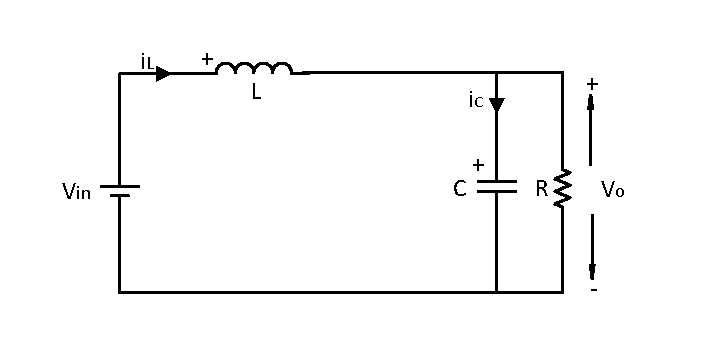
\includegraphics[width=\textwidth]{figures/aConventionalBoost/ConventionalBoostConverterOFF.pdf}
    \caption{Conventional Boost Converter Switch OFF}
	\label{fig:ConventionalBoostOFF}
\end{figure}

When the switch is OFF,
the capacitor is being charged and this is the mode when the boosting happens.

In this case we have:
\begin{equation}
	V_L = V_{in} - V_o
	\label{eq:pumpHeadModel}
\end{equation}

\begin{equation}
	i_C = i_L -\frac{V_o}{R}
	\label{eq:pumpHeadModel}
\end{equation}

\begin{figure}[H]
   \centering
   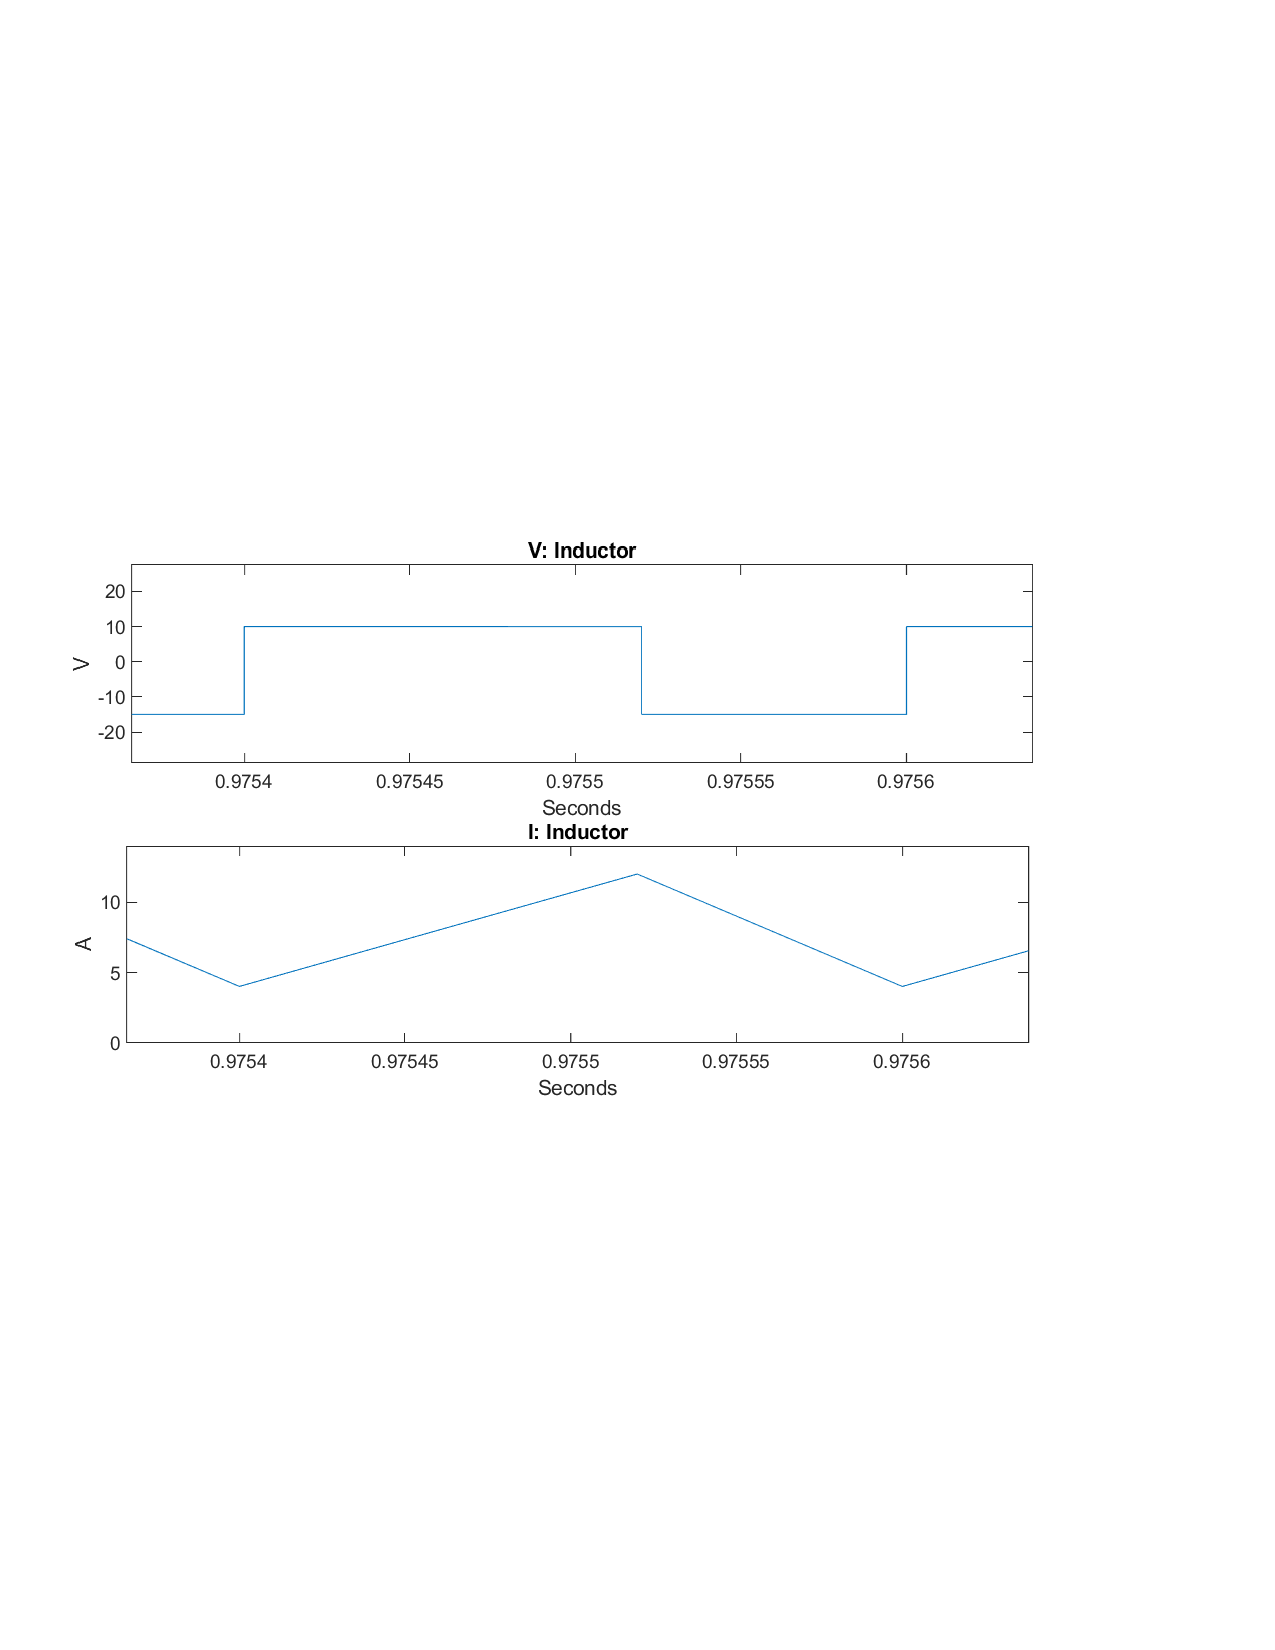
\includegraphics[width=\textwidth]{figures/aConventionalBoost/LvAndLi.pdf}
    \caption{CBC Inductor Wave Forms}
	\label{fig:ConventionalBoostOFF}
\end{figure}

\subsection{Convertion ratio}\label{sec:SON}

Based on inductor volt-second balance, the convertion ratio can be calculated:

\begin{equation}
	V_{in}D + (V_{in}-V_{out})(1-D) = 0
	\label{eq:pumpHeadModel}
\end{equation}

\begin{equation}
	\frac{V_o}{V_{in}} = \frac{1}{1-D}
	\label{eq:pumpHeadMode5}
\end{equation}

\subsection{Inductor current ripple}\label{sec:SON}

The inductor current slope for the interval from 0 to DTs can be found as:

\begin{equation}
	\frac{di_{L}(t)}{dt} = \frac{v_{L}(t)}{L} = \frac{V_{in}}{L}
	\label{eq:pumpHeadMode5}
\end{equation}

and the current slope for the interval 1 - DTs:

\begin{equation}
	\frac{di_{L}(t)}{dt} = \frac{v_{L}(t)}{L} = \frac{V_{in} - V}{L}
	\label{eq:pumpHeadMode5}
\end{equation}

The change of inductor current during the subinterval is:

\begin{equation}
	2\Delta i_L = \frac{V_{in}}{L}DT_s \Rightarrow
  \Delta i_L = \frac{V_{in}}{2L}DT_s
	\label{eq:pumpHeadMode5}
\end{equation}

The inductor should be chosen such that a desired ripple magnitude is optained.

\subsection{Capacitor voltage ripple}\label{sec:SON}



\begin{equation}
	V_{in}D + (V_{in}-V_{out})(1-D) = 0
	\label{eq:pumpHeadModel}
\end{equation}

